% Initial config
\usepackage[utf8]{inputenc}
\usepackage{glossaries-extra}

% Title and authors
\title{End of Studies Project}
\author{
    Anis, Benna\\
    \texttt{anis.benna@incedo.com}
    \and
    Firas, Jaber\\
    \texttt{firas.jaber@incedo.com}
}
\date{March 2022}

% Import packages
\usepackage{pdfpages}
\usepackage{natbib}
\usepackage{graphicx}
\usepackage{float}
\usepackage{tabularx}
\usepackage{colortbl}
\usepackage{multirow}
\usepackage{caption}
\usepackage{chngcntr}
\usepackage[hyphens]{url}
\usepackage{listings}
\usepackage{color}
\usepackage{textcomp}
\usepackage[toc,page]{appendix}
\usepackage{ragged2e}
\usepackage{enumitem}
\usepackage[parfill]{parskip} % \medskip and \noindent are not needed. See https://tex.stackexchange.com/a/74173/268270
\usepackage{fancyhdr}
\usepackage[nohints]{minitoc}
\usepackage{xcolor}
\usepackage{pdflscape}
\usepackage{xltabular}
\usepackage{array}


% Define color
\definecolor{darkgreen}{HTML}{3C6255}
\definecolor{newBlue}{HTML}{6C9BCF}
\definecolor{darkPurple}{HTML}{D25380}
\definecolor{limeGreen}{HTML}{5BB318}


% DEVONLY:
\usepackage{lipsum} % Lorem ipsum

% Glossary list
% \newglossaryentry{latex}
% {
%     name=latex,
%     description={Is a mark up language specially suited
%             for scientific documents}
% }
% \newglossaryentry{maths}
% {
%     name=mathematics,
%     description={Mathematics is what mathematicians do}
% }

% List of acronyms
\newacronym{ilg}{ILG}{Incedo Lead Generator}
\newacronym{saas}{SaaS}{Software as a Service}
\newacronym{vm}{VM}{Virtual Machine}
\newacronym{iac}{IaC}{Infrastructure as Code}

% NOTE: Using acronyms in the document
% \glsxtrlong{ilg} => Incedo Lead Generator
% \glsxtrshort{ilg} => ILG
% \glsxtrfull{ilg} => Incedo Lead Generator (ILG)

% \acrlong{ilg} \acrshort{ilg} \acrfull{ilg} can also be used but should not in our current setup.
% See https://tex.stackexchange.com/questions/318694/glossaries-acronyms-avoid-additional-entries-in-number-list-with-indexonlyfirs


% ------------- Document content ------------- %
\begin{document}

% Global config
% Color palette
\definecolor{primary}{cmyk}{0, 0.23, 0.98, 0.17}
\definecolor{secondary}{cmyk}{0.48, 0.16, 0, 0.61}
\definecolor{listinggray}{gray}{0.9}
\definecolor{lbcolor}{rgb}{0.9,0.9,0.9}

% Global Figure and Table count
\counterwithout{figure}{chapter}
\counterwithout{table}{chapter}

% Chapter name on each page
\pagestyle{fancy}
\lhead{}
\chead{}
\renewcommand{\headrulewidth}{0pt} % Remove the underline
\setlength{\headheight}{15pt}

% Initialize the mini toc at the beginning of each chapter
% More config https://tex.stackexchange.com/a/4858/268270
\dominitoc[n]
\nomtcrule
\setcounter{minitocdepth}{1}

% Code highlighting for supported languages
% https://en.wikibooks.org/wiki/LaTeX/Source_Code_Listings#Supported_languages
\lstset{
    backgroundcolor=\color{lbcolor},
    tabsize=4,
    rulecolor=,
    language=matlab,
    basicstyle=\scriptsize,
    upquote=true,
    aboveskip={1.5\baselineskip},
    columns=fixed,
    showstringspaces=false,
    extendedchars=true,
    breaklines=true,
    prebreak = \raisebox{0ex}[0ex][0ex]{\ensuremath{\hookleftarrow}},
    frame=single,
    showtabs=false,
    showspaces=false,
    showstringspaces=false,
    identifierstyle=\ttfamily,
    keywordstyle=\color[rgb]{0,0,1},
    commentstyle=\color[rgb]{0.133,0.545,0.133},
    stringstyle=\color[rgb]{0.627,0.126,0.941},
}

% Add custom language support for yaml
% https://tex.stackexchange.com/questions/152829/how-can-i-highlight-yaml-code-in-a-pretty-way-with-listings
\newcommand\YAMLcolonstyle{\color{red}\mdseries}
\newcommand\YAMLkeystyle{\color{black}\bfseries}
\newcommand\YAMLvaluestyle{\color{blue}\mdseries}
\makeatletter
\newcommand\language@yaml{yaml}
\expandafter\expandafter\expandafter\lstdefinelanguage
\expandafter{\language@yaml}
{
keywords={true,false,null,y,n},
keywordstyle=\color{darkgray}\bfseries,
basicstyle=\YAMLkeystyle,                                 % assuming a key comes first
sensitive=false,
comment=[l]{\#},
morecomment=[s]{/*}{*/},
commentstyle=\color{purple}\ttfamily,
stringstyle=\YAMLvaluestyle\ttfamily,
moredelim=[l][\color{orange}]{\&},
moredelim=[l][\color{magenta}]{*},
moredelim=**[il][\YAMLcolonstyle{:}\YAMLvaluestyle]{:},   % switch to value style at :
morestring=[b]',
morestring=[b]",
literate =    {---}{{\ProcessThreeDashes}}3
{>}{{\textcolor{red}\textgreater}}1
{|}{{\textcolor{red}\textbar}}1
{\ -\ }{{\mdseries\ -\ }}3,
}
\lst@AddToHook{EveryLine}{\ifx\lst@language\language@yaml\YAMLkeystyle\fi}
\makeatother
\newcommand\ProcessThreeDashes{\llap{\color{cyan}\mdseries-{-}-}}
% Usage example
% \begin{lstlisting}[language=yaml]
%     stages:
%       - test
%       - buildPublish
%       - deploy
% \end{lstlisting}


% Include the cover page

\includepdf[]{src/assets/pdfs/cover-page.pdf}

% Set page numbering to roman for initial pages
\pagenumbering{roman}
\setcounter{page}{1}

% Dedication and acknowledgments
% \section*{Dedication}
\lipsum[1-3]
\newpage

\section*{Dedication}
\lipsum[1-3]
\newpage
 % Optional
\section*{Acknowledgments}
We would like to take a moment to thank all of those involved in finalizing this work, whether directly or indirectly.

% Thanking the Incedo team
Our profound gratitude goes to the entire \textbf{Incedo Services GmbH team} for their warm welcome, invaluable support and for accompanying us throughout this wonderful journey.
Special thanks to our company supervisor and product owner \textbf{Mr. Manuel Schulze} who has been very involved with us almost daily throughout the long period of the internship, his trust in us has truly allowed us to come very far during this project.
We also appreciate \textbf{Wael Jaber} for initially showing us the ropes and for his continuous guidance.
Our deepest gratefulness also goes to \textbf{Mr. Robert Könitz} and \textbf{Mr. Tobias Schulze} for their huge efforts in contributing to our weekly mentoring sessions amongst other things, their input has truly been a huge source of knowledge for both of us and will be forevermore.
We would also like to thank both of \textbf{Mrs. Mai Ly Moll} and \textbf{Mrs. Xenia Harter} for their efforts in business development and for organizing the delightful team events that we gladly had the occasion to participate in, as well as for their almost daily engagements that don't fall short from our supervisor's. We also extend our thanks to the rest of the Incedo team \textbf{Mr. Joachim Liedtke}, \textbf{Mr. Mohamed Elloumi} and \textbf{Mr. Gabor Kluge}.

% Thanking the University supervisor
We also wish to acknowledge the great support of our university supervisor \textbf{Mrs. Mahassen Khemiri} for her assistance, availability and valuable spot-on advice.
Her faith in us has truly allowed us to keep working on this project stress-free while confident this report will turn out better than initially intended.

Our heartfelt appreciation goes to the jury members who agreed to evaluate our work and we hope they find it up to standard.
We equally thank all of the teachers of the Higher Institute of Technological Studies of Nabeul (ISETN) who contributed to our education during these wonderful two and a half years.

% \medskip
% \noindent We would also like to take this opportunity to express how joyful we are to keep working as official permanent team members of Incedo!

\newpage


% Abstract or TL;DR
\section*{Abstract (TL;DR)}
\lipsum[1-3]
\newpage


% Print the acronyms list
\printunsrtglossaries
\newpage

% Tables
\renewcommand{\contentsname}{Table of Contents}
\tableofcontents
\listoffigures \mtcaddchapter % https://tex.stackexchange.com/questions/155177/how-to-add-the-word-figure-to-the-list-of-figures
\listoftables \mtcaddchapter % https://tex.stackexchange.com/questions/79869/first-chapter-after-list-of-tables-starts-on-page-2-should-be-1
\clearpage

% Set page numbering to Arabic for main content
\pagenumbering{arabic}

% Include the main app
% Main Document
\maketitle

\chapter{ General framework}
\setcounter{secnumdepth}{3}
\newpage

\section*{Introduction}
\addcontentsline{toc}{section}{Introduction}
This chapter introduces the general context of this report. We start by presenting the frame of the project as well as the host company. Then comes the enumeration of the problems which led to the realization of the project. We wrap it up by defining the methodology we’ve followed to carry out our work.

\section{General framework of the internship}
\addcontentsline{toc}{section}{General framework of the internship}
This project was carried out within the frame of obtaining a bachelor’s degree in Computer Science at the Higher Institute of Technological studies of Nabeul. The internship took place fully remotely at Incedo Services GmbH for five months starting from the 1st of February 2022 to the 30th of June 2022 with the purpose of further developing the existing project as well as slowly migrating it to a micro-services architecture.

\section{Company overview}
\addcontentsline{toc}{section}{Company overview}
This section introduces the host company and its offered services.
\subsection{About Incedo}
\subsection{Incedo Services}

\section{Stating the problem}
\addcontentsline{toc}{section}{Company overview}
Incedo -having ambitious goals to grow over the next 2 to 4 years- wants to win new clients and strategically develop the existing ones. Winning new clients starts with generating new leads. Previously, Incedo has worked with an Austrian start-up (motion group) that provides automated lead generation through LinkedIn at the cost of 0.85 € per requested contact in LinkedIn. Although one big project was closed and several leads were generated, Incedo started using the LinkedIn Sales Navigator with a more targeted approach, but nevertheless wanted to automate the approach and increase its outreach.
Having launched the first version of the ILG (Incedo Lead Generator) as a SaaS (Software as Service), Incedo was satisfied for a while. Over the time however, as more and more clients were interested in the ILG, the current architecture couldn’t handle the load properly.

\section{Assessment of the case}
\addcontentsline{toc}{section}{Assessment of the case}
\subsection{Describing the work procedure}
The work on any project must first of all be preceded by a thorough study of the existing ones which undermines the strengths and weaknesses of the current system, as well as the business decisions that should be taken into account during the conception as well as the realization.
\subsection{Criticizing the current state}
After studying the existing, we can determine its limitations:
\begin{itemize}
	\item Bugs always tend to happen whenever the LinkedIn website changes (due to scraping). 
	\item Since cron jobs are running for the whole day, bugs are hard to respond to fast enough because we can only deploy once at the end of day. 
	\item It is hard to test the whole workflow because of how the app works (looking for certain changes in the LinkedIn interface after certain buttons are clicked for example) meaning that the dev environment is lacking.
	\item It cannot scale well enough since the whole application is deployed on a single server.
\end{itemize} 
\subsection{Proposed solution}
% NOTE: Fix New Paragraph identation
The solution to these problems is refactoring the whole application to separate sub applications (microservices) where the automation and scraping processes can be scaled independently of the other parts of the application.

\medskip
This way, it will be easier to maintain and scale the different codebases as well as respond faster to bugs and know exactly what caused them in the first place.


\newpage
\section{Assessment of the case}
\addcontentsline{toc}{section}{Assessment of the case}
\subsection{Agile methodology}
Agile is a structured and iterative approach to project management and product development. It recognizes the volatility of product development, and provides a methodology for self-organizing teams to respond to change without going off the rails.
\subsection{Scrum methodology}
Scrum teams commit to completing an increment of work, which is potentially shippable, through set intervals called sprints. Their goal is to create learning loops to quickly gather and integrate customer feedback. Scrum teams adopt specific roles, create special artifacts, and hold regular ceremonies to keep things moving forward.
\subsection{Kanban methodology}
Kanban is all about visualizing your work, limiting work in progress, and maximizing efficiency (or flow). Kanban teams focus on reducing the time a project takes (or user story) from start to finish. They do this by using a kanban board and continuously improving their flow of work.
\subsection{The choice for ILG}
Kanban is based on a continuous workflow structure that keeps teams nimble and ready to adapt to changing priorities. Work items—represented by cards— are organized on a kanban board where they flow from one stage of the workflow(column) to the next. Common workflow stages are To Do, In Progress, In Review, Blocked, and Done. And since this project is very susceptible to changes from outside (LinkedIn), Kanban offered more flexibility than Scrum so that’s why the team went with it instead.


\chapter{ State of the art }
\setcounter{secnumdepth}{3}
\newpage

% ----------------------- Introduction ----------------------- %
\section*{Introduction}
\addcontentsline{toc}{section}{Introduction}
This chapter will present and study various concepts such as Automation, Web Scraping, Version Control, DevOps, State Machine with an emphasis on the DevOps terminology such as the CI/CD pipelines. We will talk about the most used tools in the market as well as which ones we settled on after making a comparison.

\section{Automation \& Web Scraping concepts}
\addcontentsline{toc}{section}{Automation & Web Scraping concepts}
\subsection{Automation}
At its core, automation is leaving menial and recurring tasks to the automaton (or machine) in order to do more meaningful work as a human in the meantime. Implementing automation improves the efficiency, reliability and the speed of tasks that previously took humans a lot of time.
\subsection{Web Scraping}
Web scraping is the process of automatically extracting content and data from a website. Although data extraction is done in a brute way by reading texts from HTML elements, it is used in a variety of legitimate digital businesses like search engines, price comparison sites and market research companies. So contrary to what some might think, web scraping is completely legal.
\subsection{Relationship between the two}
Web scraping simplifies the process of extracting data and the automation process helps repeating the recurring task of extraction. As a result, the combination of scraping data, storing it and automating the whole process is getting very popular, especially with new technologies and tools arising in order to do just that.

\newpage

% ----------------------- DevOps ----------------------- %
\section{DevOps}
\addcontentsline{toc}{section}{DevOps}

\subsection{Definition}
DevOps is the set of practices, techniques and tools used to speed up the Software Development Lifecycle (SDL) by bringing together two historically separate functions of development and operations.

\medskip
Development refers to writing code and software, whereas operations refer to provisioning servers, configuring them as well as deploying the apps to them, amongst other things.

\medskip
DevOps teams focus on automating all of the above. The key terminologies around DevOps are Continuous Integration, Continuous Delivery and Infrastructure As Code (IAC).

\subsection{Lifecycle}
\begin{center}
	\includegraphics[width=9cm, height=5cm]{src/assets/images/devops.png}
\end{center}
\subsection{Container management}
Containers have become an integral part of DevOps over the past couple of years but what is a container exactly and how do we manage them?
\subsubsection*{What is a container ?}
Simply said; container is a packaging format for software applications that are akin to a very lightweight virtual machine which always executes in an isolated environment. What this implies is that said containers can be easily copied to and run on different machines with high reliability, lower costs and high efficiency.
\subsubsection*{What is container management ?}
Container management is the process for automating the creation, deployment and scaling of containers. Container management tools such as Docker and Podman facilitate the addition, replacement and organization of containers.

% ----------------------- Mincroservices ----------------------- %
\section{Microservices}
\addcontentsline{toc}{section}{Microservices}

\subsection{Definition}
Microservices are an architectural and organizational approach to software development where software is composed of small independent services that communicate over well-defined APIs. These services are owned by small, self-contained teams.

\medskip
Microservices architectures make applications easier to scale and faster to develop, enabling innovation and accelerating time-to-market for new features.
\begin{center}
	\includegraphics[width=10cm, height=7cm]{src/assets/images/microservices.png}
\end{center}
\subsection{Characteristics of Microservices}
\begin{itemize}
	\item \textbf{Autonomous :} Each component service in a microservices architecture can be developed, deployed, operated, and scaled without affecting the functioning of other services. Services do not need to share any of their code or implementation with other services. Any communication between individual components happens via well-defined APIs.
	\item \textbf{Specialized :} Each service is designed for a set of capabilities and focuses on solving a specific problem. If developers contribute more code to a service over time and the service becomes complex, it can be broken into smaller services.
\end{itemize}

\subsection{Benefits of Microservices}
\begin{itemize}
	\item \textbf{Agility :} Microservices foster an organization of small, independent teams that take ownership of their services. Teams act within a small and well understood context, and are empowered to work more independently and more quickly.
	\item \textbf{Flexible Scaling :} Microservices allow each service to be independently scaled to meet demand for the application feature it supports. This enables teams to right-size infrastructure needs, accurately measure the cost of a feature, and maintain availability if a service experiences a spike in demand.
	\item \textbf{Easy Deployment :} Microservices enable continuous integration and continuous delivery, making it easy to try out new ideas and to roll back if something doesn’t work. The low cost of failure enables experimentation, makes it easier to update code, and accelerates time-to-market for new features.
	\item \textbf{Technical Freedom :} Microservices architectures don’t follow a “one size fits all” approach. Teams have the freedom to choose the best tool to solve their specific problems. As a consequence, teams building microservices can choose the best tool for each job.
	\item \textbf{Reusable Code :} Dividing software into small, well-defined modules enables teams to use functions for multiple purposes. A service written for a certain function can be used as a building block for another feature. This allows an application to bootstrap off itself, as developers can create new capabilities without writing code from scratch.
	\item \textbf{Resilience :} Service independence increases an application’s resistance to failure. In a monolithic architecture, if a single component fails, it can cause the entire application to fail. With microservices, applications handle total service failure by degrading functionality and not crashing the entire application.
\end{itemize}

% ----------------------- Comparative Analysis ----------------------- %
\section{Comparative Analysis}
\addcontentsline{toc}{section}{Comparative Analysis}

In order to get started with our project, we need a wide range of tools that deal with the following areas; version control, orchestration between containers, browser automation as well as scheduled automation. For that, we did a comparative study on some of the tools the market provides.

\subsection{Version Control: Git vs SVN}
The most used tools for version control are Git and SVN. Here is a table comparing both tools.
\begin{table}[H]
	\renewcommand{\arraystretch}{1.5}%
	\caption{Comparative study between existing methodologies}
	\centering
	\medskip
	\begin{tabularx}{1\textwidth} {
			| >{\hsize=.5\hsize\linewidth=\hsize\centering\arraybackslash}X
			| >{\hsize=1.25\hsize\linewidth=\hsize\centering\arraybackslash}X
			| >{\hsize=1.25\hsize\linewidth=\hsize\centering\arraybackslash}X |}
		\hline
		\rowcolor{primary} & \textbf {Description}                                                                                                                          & \textbf {Advantages}                                                                                                                                                           \\
		\hline
		\textbf{Git}       & Git is a distributed version control system which means that when coloning a repository, you get a copy of the entire history of that project. & Git has what's called a staging area. This means that even if you made over a 100 changes, they can be broken down to 10 commits each with their own comments and description. \\
		\hline
		\textbf{SVN}       & SVN or Subversion is a centralized version control system. Meaning that there is always a single version of the repository that you checkout.  & SVN has one central repository – which makes it easier for managers to have more of a top down approach to control, security, permissions, mirrors, and dumps.                 \\
		\hline
	\end{tabularx}
\end{table}
At the end, both are great options. However, we will be using Git which is the VCS the company uses.

\subsection{Container management: Docker vs Podman}
Although Docker is widely popular, Podman is also taking its share from the market. Especially on Redhat systems.
\begin{table}[H]
	\renewcommand{\arraystretch}{1.5}%
	\caption{Comparative study between existing methodologies}
	\centering
	\medskip
	\begin{tabularx}{1\textwidth} {
			| >{\hsize=.7\hsize\linewidth=\hsize\centering\arraybackslash}X
			| >{\hsize=1.15\hsize\linewidth=\hsize\centering\arraybackslash}X
			| >{\hsize=1.15\hsize\linewidth=\hsize\centering\arraybackslash}X |}
		\hline
		\rowcolor{primary} \textbf {Aspect} & \textbf {Docker}                                                                                                                              & \textbf {Podman}                                                                                                                                               \\
		\hline
		\textbf {Definition}                & \multicolumn{2}{Muasdlti-column}                                                                                                                                                                                                                                                                               \\
		\hline
		\textbf {Technology}                & SVN or Subversion is a centralized version control system. Meaning that there is always a single version of the repository that you checkout. & SVN has one central repository – which makes it easier for managers to have more of a top down approach to control, security, permissions, mirrors, and dumps. \\
		\hline
		\textbf {Architecture}              & SVN or Subversion is a centralized version control system. Meaning that there is always a single version of the repository that you checkout. & SVN has one central repository – which makes it easier for managers to have more of a top down approach to control, security, permissions, mirrors, and dumps. \\
		\hline
	\end{tabularx}
\end{table}
As a result, we will also be sticking to Docker in this project.

\chapter{Analysis and specification of requirements:}
\setcounter{secnumdepth}{3}
\newpage

\section{Analysis}
\addcontentsline{toc}{section}{Analysis}

\section{Requirements}
\addcontentsline{toc}{section}{Requirements}

\subsection{SprintOne}
\addcontentsline{toc}{subsection}{SprintOne}

\subsubsection{Sprint Story and Objective}
\addcontentsline{toc}{subsection}{The Story and Objective}

\subsubsection{Sprint Analysis}
\addcontentsline{toc}{subsection}{Sprint Analysis}

\subsubsection{Sprint Kanban Board}
\addcontentsline{toc}{subsection}{Sprint Kanban Board}

\subsubsection{Sprint Review}
\addcontentsline{toc}{subsection}{Sprint Review}

% TODO : CHANGE_ME
\subsection{SprintTwo}
\addcontentsline{toc}{subsection}{SprintOne}

\subsubsection{Sprint Story and Objective}
\addcontentsline{toc}{subsection}{The Story and Objective}

\subsubsection{Sprint Analysis}
\addcontentsline{toc}{subsection}{Sprint Analysis}

\subsubsection{Sprint Kanban Board}
\addcontentsline{toc}{subsection}{Sprint Kanban Board}

\subsubsection{Sprint Review}
\addcontentsline{toc}{subsection}{Sprint Review}

% TODO : CHANGE_ME
\subsection{SprintThree}
\addcontentsline{toc}{subsection}{SprintOne}

\subsubsection{Sprint Story and Objective}
\addcontentsline{toc}{subsection}{The Story and Objective}

\subsubsection{Sprint Analysis}
\addcontentsline{toc}{subsection}{Sprint Analysis}

\subsubsection{Sprint Kanban Board}
\addcontentsline{toc}{subsection}{Sprint Kanban Board}

\subsubsection{Sprint Review}
\addcontentsline{toc}{subsection}{Sprint Review}

\chapter{Realization :}
\setcounter{secnumdepth}{3}
\newpage

\section{General architecture}
\addcontentsline{toc}{section}{General architecture}

\section{Work environment}
\addcontentsline{toc}{section}{Work environment}

\section{Difficulties encountered}
\addcontentsline{toc}{section}{Difficulties encountered}
\chapter{Conclusion :}
\setcounter{secnumdepth}{3}
\newpage

\section{General conclusion}
\addcontentsline{toc}{section}{General conclusion}



% Generate a webography, for more styles
% see - https://www.overleaf.com/learn/latex/Bibtex_bibliography_styles#Table_of_stylename_values
\renewcommand\bibname{Webography}
\bibliographystyle{plain}
\bibliography{references}
\clearpage

% % Set page numbering to alphabetic for appendices
\pagenumbering{alph}
\setcounter{page}{0}

% Very big diagrams, pictures or schemas go here
% List of appendices
\begin{appendices}
    % Appendix a
    \section{MyApp management}
    \begin{figure}[H]
        \centering
        \makebox[\textwidth]{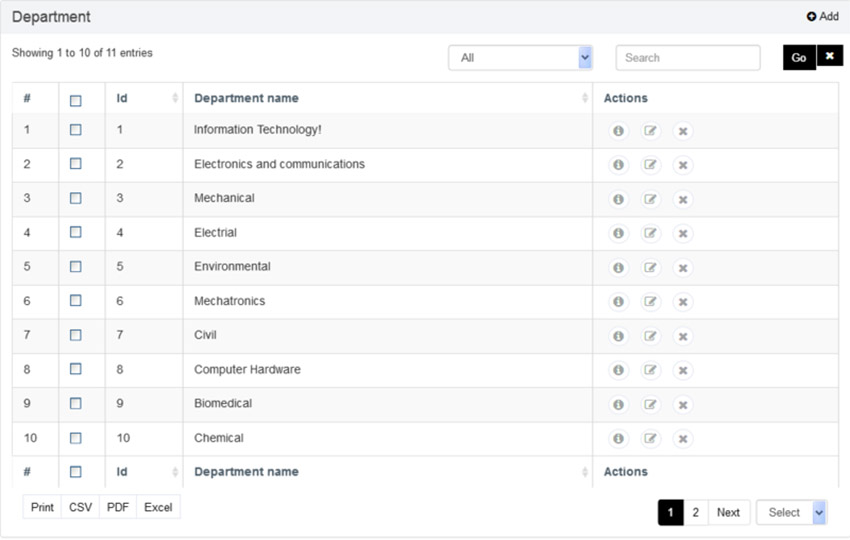
\includegraphics[width=12cm]{src/assets/screenshots/crud-gen-example-1.jpg}}
        \caption*{Show list}
    \end{figure}
    \begin{figure}[H]
        \centering
        \makebox[\textwidth]{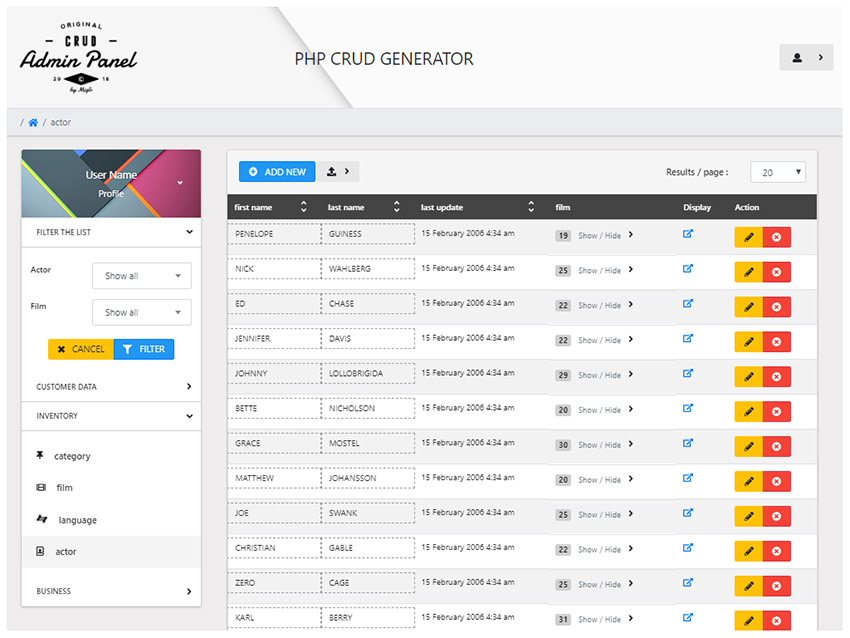
\includegraphics[width=12cm]{src/assets/screenshots/crud-gen-example-2.jpg}}
        \caption*{Filter list}
    \end{figure}

    % Appendix b
    \section{Kubernetes dashboard}
    The Kubernetes dashboard is a web based UI for Kubernetes clusters.
    It allows the management of applications running in the cluster.
    \begin{figure}[H]
        \centering
        \makebox[\textwidth]{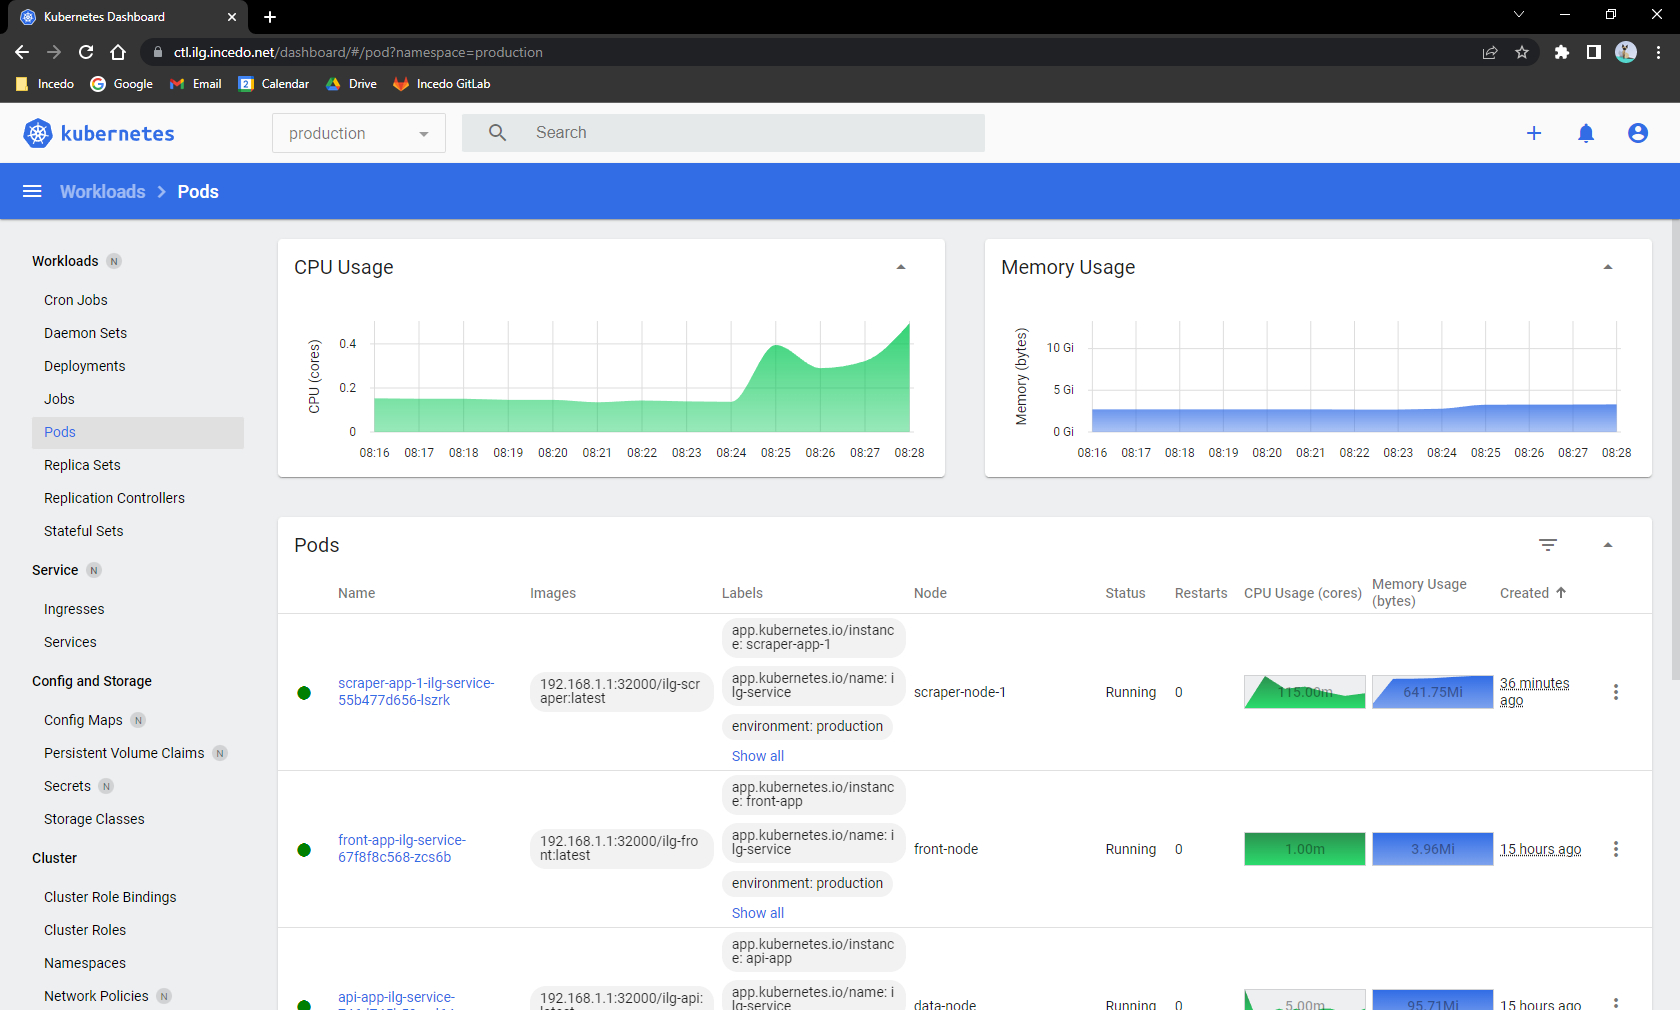
\includegraphics[width=\linewidth]{src/assets/images/kubernetes-dashboard-pods.JPG}}
        \caption*{Monitoring the pods with the Kubernetes dashboard}
    \end{figure}
    \begin{figure}[H]
        \centering
        \makebox[\textwidth]{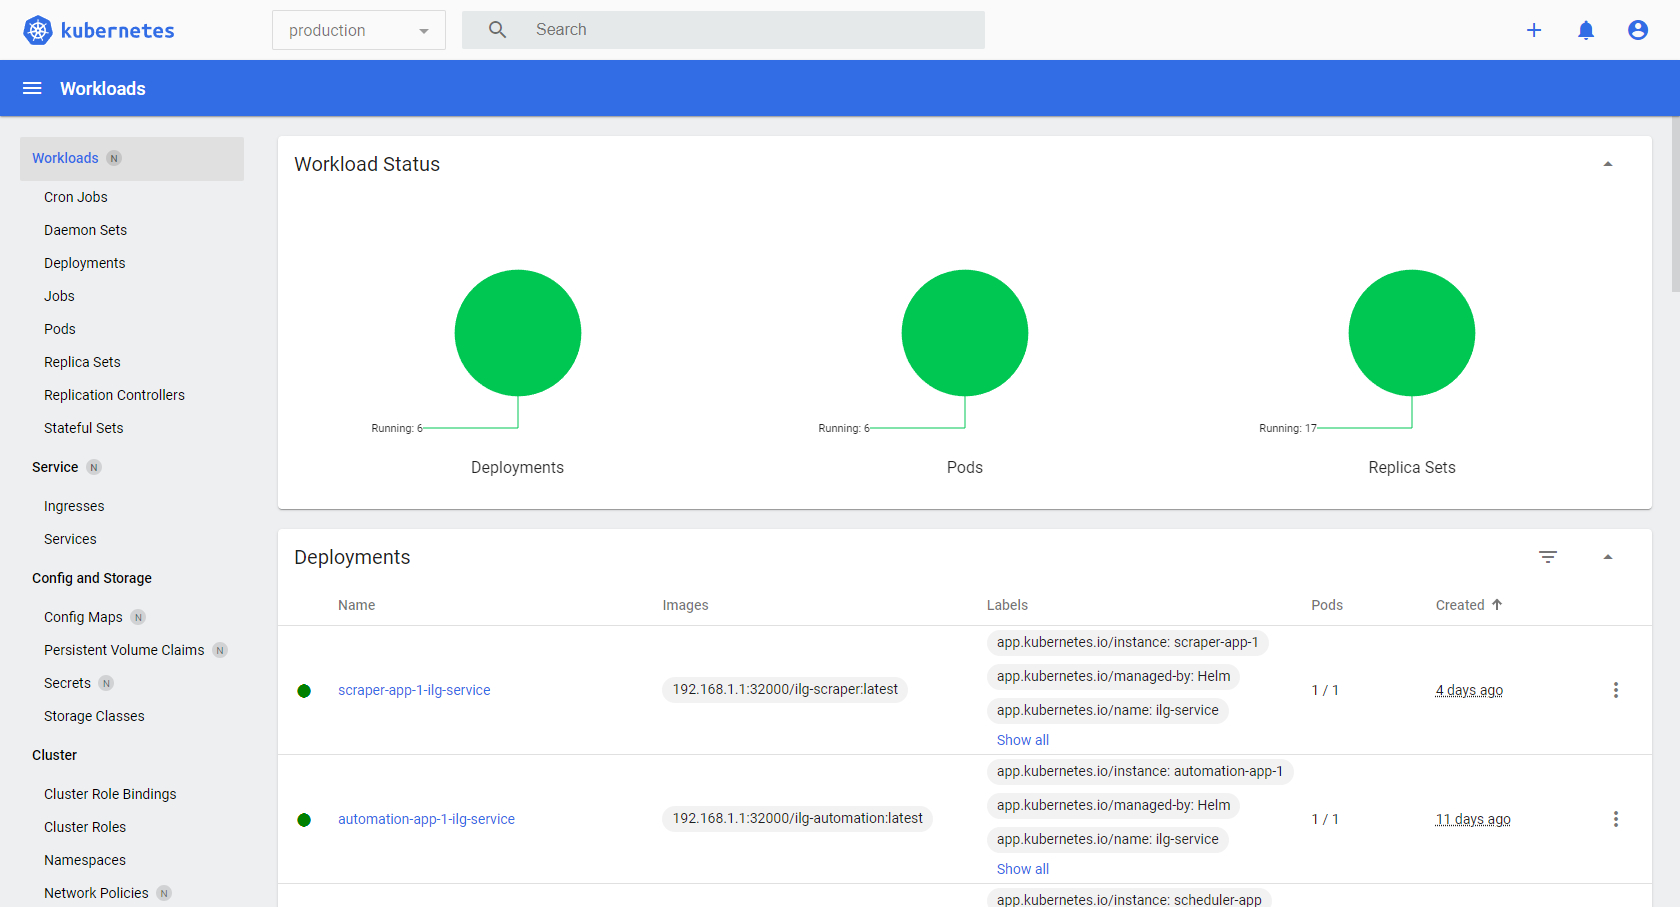
\includegraphics[width=\linewidth]{src/assets/images/kubernetes-dashboard-workloads.JPG}}
        \caption*{Monitoring the workloads with the Kubernetes dashboard}
    \end{figure}
    \newpage
\end{appendices}


\end{document}
% ------------- Document content ------------- %
